\documentclass{acm_proc_article-sp}

\usepackage{graphicx} %package to manage images
\graphicspath{ {images/} }

\usepackage[rightcaption]{sidecap}

\usepackage{wrapfig}

\begin{document}

\title{Project: Seismic Data Analysis and Ground Motion Visualization}

\numberofauthors{4} 
\author{
\alignauthor
Tony Liu\titlenote{PhD student at Indiana University}\\
       \affaddr{Indiana University}\\
       \affaddr{Bloomington, IN}\\
\email{xl41@indiana.edu}
}

\date{30 September 2016}


\maketitle
\begin{abstract}
We propose to deploy a seismic data processing environment with no-relational database (MongoDB), analyze the seismic data and visualize a ground motion event.
\end{abstract}

\keywords{Seismology, MongoDB, GMV} % NOT required for Proceedings

\section{Introduction}

The science of seismology is awash in data. In the past 20 years the quantity of data available for the typical seismology research project has grown by at least three orders of magnitude.  Our field is well fed by Incorporated Research Institutions for Seismology (IRIS~\cite{IRIS}) that has done a fantastic job of building and maintaining an accessible archive of these data.  The problem this project addresses, in fact, would not exist were it not for the ready availability of this sea of data from IRIS.  The fundamental community problem this project addresses is that while the available data has grown by many orders of magnitude there have been no major software innovations for processing this ocean of data.  All the standard software tools used by the research community are founding on computing concepts that were leading edge ideas twenty (Antelope~\cite{Antelope}) to thirty (Seismic Analysis Code) years or more ago.  The key premise of this proposal is that this creaky infrastructure is seriously limiting scientific advances in seismology and has imposed a throttle on scientific advances from Earthscope.  The seismology community is like a group of young children given access to the Library of Congress.  We can only read and use a tiny fraction of the information in this vast pile of new data.  

A second principle is that the project proposed here is the engineering part of a strategic research project to address two elements needed to build a more scalable advanced processing system for seismology: (1) a meta-data handling system for data processing that is flexible, extensible, and capable of storing the full range ancillary parameters that define a data processing flow, and (2) a scalable, approachable system for implementing algorithms in the modern world of high performance computing characterized by massively parallel systems.


\section{Implementation}

The focus of this project is research to consider the efficacy of two technologies for improving passive array data processing:
1.	The seismic data processing flow in Figure 1 is a typical example of an embarrassingly parallel problem.  The reason is that with this data flow model each seismogram or group (ensemble) of seismogram is processed by the same chain of algorithms each defined by the same set of control parameters.  This type of problem is known to be well suited to the concept of Map-Reduce as implemented in software packages like Hadoop and Spark.  

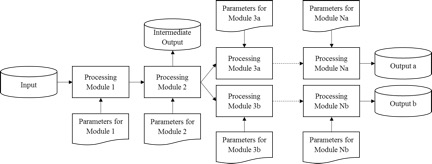
\includegraphics[scale=0.5]{Picture1}

Figure 1 Generic work flow for processing of seismic reflection data. The work flow commonly begins with the input of raw data and ends with the output of processed results. The processing modules represent one component of processing such as deconvolution, velocity analysis and migration.  Each processing module is independent, because the input and output conform a predefined format.  Therefore, the intermediate result of each module could be saved and retrieved later.  Most systems provide a means to fork into multiple work flows.  

2.	We propose to use a NoSQL database (MongoDB) as the framework to handle all meta-data related to a collection of seismogram.  The idea is to use a common NoSQL database to manage not just conventional header information, but also input parameters for all processes and log information from each processing module. 

For implementation detail of this project, there are three parts:
Seismic data includes meta-data and waveforms, while meta-data is stored and managed by Antelope and waveforms are stored on the file system. The data set is downloaded from USArray, IRIS. The waveforms are encrypted as structured binary files called MiniSEED ~\cite{MiniSeed}. The files need to be loaded into Antelope and file system. 

To extract, transfer and load the seismic data from Antelope to MongoDB, tool needs to be developed to use the Antelope Python API to read and manipulate the meta-data from Antelope and ObsPy~\cite{ObsPy} to read and decrypt the MiniSEED file from the file system and extract the waveforms from them. In order to store all the information, PyMongo~\cite{PyMongo} (MongoDB Python API) is used to access MongoDB and pickle (Python object serialization) is used to serialize the seismic waveform data so they can be stored in GridFS, another component for storage within MongoDB. 
 
After the environment is set, I deploy sharding~\cite{shard} for MongoDB to have a better data scalability and automatic backup. Furthermore, I implement DSP algorithms on filtering and down-sampling.

After some analysis on the event I selected, I visualize the processed seismic data of that event with D3JS.


\section{Artifacts}

Part I:
Recipe on cluster deployment and configuration
This part is called recipe.ipynb

Part II:
Python Program to migrate seismic data from Antelope to MongoDB
This part is under folder loader, include loader.sh and transfer.sh. Loader is to migrate meta-data from Antelope to MongoDB. Transfer is to migrate waveform from file system to GridFS within MongoDB.

Part III:
Notebook Recipe on seismic data analysis
This part is call analysis.ipynb, this is under folder visualization. Once it's done, it will generate four javascript file including all the seismic data for next step.

Part IV:
HTML file to demonstrate Ground Motion Visualization
This part is under folder visualization. Ground motion visualization is implemented with an HTML file and the javascript file generate by the previous step. I associate the red and larger dot with positive amplitude, the blue and smaller dot with negative amplitude. The web page will load the data from javascript file and replay the earthquake event I select frame by frame like a movie. Also, I add some small features like change the color related to the dots, and increase the speed for the visualization.

\bibliographystyle{abbrv}
\bibliography{proposal}

%\balancecolumns 

\end{document}

